\chapter{Extended phase model}

In Section~\ref{sec:mqfmfromphase} it was shown how a cubic phase function could
be postulated from two connected measurements (see
Section~\ref{sec:partialtracking}) giving a cubic phase polynomial. Here we will
demonstrate how to include the additional phase polynomial coefficients
estimated using DDM in calculating a phase function. In a later section we will
compare the synthesis quality of the classical McAulay \textendash Quatieri
approach with our new method.

\section{Cubic phase polynomial\label{sec:cubicphasepoly} }

In this section we describe how to obtain a cubic phase polynomial from
local estimations of the coefficients of a quadratic phase polynomial.

A complex sinusoid with cubic phase has the following form:
\begin{equation}
    \label{eq:cubicphasepoly}
    \phi(n) = \exp \left(c_3 n^{3} + c_2 n^{2} + c_1 n + c_0 \right)
\end{equation}
One with quadratic phase has this form:
\begin{equation}
    \label{eq:quadraticphasepoly}
    x(n) = \exp \left(a_2 n^{2} + a_1 n + a_0 \right)
\end{equation}
with $c_{i} \in \mathbb{C}$ and $a_{i} \in \mathbb{C}$.

We can estimate the coefficients of Equation~\ref{eq:quadraticphasepoly} using the DDM. From
Equation~\ref{eq:ddmsyseq}, we define the three functions
\begin{equation}
    X_{p_{1}} \left( \tau, k \right)
    =
    \sum_{m=0}^{M-1} w(m) x(m + \tau) \exp(-j 2 \pi \frac{k m}{M})
\end{equation}
\begin{equation}
    X_{p_{2}} \left( \tau, k \right)
    =
    \sum_{m=0}^{M-1} 2 m w(m) x(m + \tau) \exp(-j 2 \pi \frac{k m}{M})
\end{equation}
\begin{equation}
    X_{w^{\prime}} \left( \tau, k \right)
    =
    -j 2 \pi \frac{k}{M} X_{p_{1}} \left( \tau , k \right) + 
    \sum_{m=0}^{M-1} \frac{dw}{dn}(m) x(m + \tau) \exp(-j 2 \pi \frac{k m}{M})
\end{equation}
Where $M$ is the length of the window and $k$ is the frequency ``bin". We also
only consider $x$ at the samples $m = [0, \dotsc, M-1]$ because we can always
shift the time reference to view an arbitrary contiguous segment of signal with
these indices.

We then find $k^{\ast}$ such that $X_{p_{1}}$ is maximum. If multiple components
are present in the signal and are sufficiently separated in frequency, we can
split the signal up into frequency bands and find local maxima. A technique for
doing so is described in \cite[p.~42]{serra1989system}. To have a system of equations
with a unique solution, take the two adjacent bins $k-1$ and $k+1$ to have
enough unique atoms for Equation~\ref{eq:ddmsyseq}. These bins
should only contain energy from the component whose parameters we are interested
in measuring \textemdash this is true if the components are adequately separated
in time and frequency. We could choose only two bins to have a non-singular
system, and there are many possibilities for choosing different atoms
\cite[p.~4639]{betser2009sinusoidal}. We choose three to have improved
estimation accuracy in situations where components are adaquately separated in
frequency. Then $a_2$ and $a_1$ can be determined by solving the linear system
\[
    \begin{pmatrix}
        X_{p_{1}} \left( \tau, k^{\ast} - 1 \right) & X_{p_{2}} \left( \tau, k^{\ast} - 1 \right) \\
        X_{p_{1}} \left( \tau, k^{\ast} \right) & X_{p_{2}} \left( \tau, k^{\ast} \right) \\
        X_{p_{1}} \left( \tau, k^{\ast} + 1 \right) & X_{p_{2}} \left( \tau, k^{\ast} + 1 \right)
    \end{pmatrix}
    \begin{pmatrix}
        a_1 \\
        a_2
    \end{pmatrix}
    =
    \begin{pmatrix}
        X_{w^{\prime}} \left( \tau, k^{\ast} - 1 \right) \\
        X_{w^{\prime}} \left( \tau, k^{\ast} \right) \\
        X_{w^{\prime}} \left( \tau, k^{\ast} + 1 \right)
    \end{pmatrix}
\]
With $a_{1}$ and $a_{2}$ determined, we can use Equation~\ref{eq:ddmestc0} to
estimate $a_0$. We will write $a^{\tau}_{i}$ to refer to coefficient $i$
determined at time $\tau$. Once the $\boldsymbol{a}^{\tau}$ have been determined
at two times $\tau_{0}$ and $\tau_{1}$, with $H = \tau_{1} - \tau_{0}$ and these
times have between determined as connected (see
Section~\ref{sec:partialtracking}), we can write a system of equations
to determine an interpolating cubic phase polynomial. To avoid numerical
instabilities and for simplicity, we shift the time origin so that $\tau_{0} =
0$. This means $c_0 = \Im \left\{ a^{\tau_0}_{0} \right\}$. To reduce the size
of the system, we require that 
\[
    \frac{d \phi}{d n} \left(\frac{H}{2} \right)
    =
    \frac{1}{2}
    \left( \Im \left\{ a^{\tau_0}_{1} \right\} + \Im \left\{ a^{\tau_1}_{1}
    \right\} \right)
\]
and
\[
    \frac{d^{2} \phi}{d n^{2}} \left(\frac{H}{2}
    \right)
    =
    \frac{1}{2} \left( \Im \left\{ a^{\tau_0}_{2} \right\} + \Im \left\{
    a^{\tau_1}_{2} \right\} \right)
\]
i.e., the frequency and first-order frequency modulation in the middle of the
segment are the average of the two measured coefficients. Finally we require
\[
    \phi \left( H \right)
    =
    \Im \left\{ a^{\tau_1}_{0} \right\} - \Im \left\{ a^{\tau_0}_{0} \right\}
    + 2 \pi U^{\ast}
\]
where $U^{\ast} \in \mathbb{Z}$ is determined to minimize
Equation~\ref{eq:minfmmq}, in this case:
\begin{equation}
    \label{eq:minfmcubic}
    \tilde{U} = \argmin_{U} \int_{0}^{H} \left(
    6 c_3 t + 2 c_2 \right)^{2} dt
\end{equation}
which is then rounded to the nearest integer to give $U^{\ast}$. To summarize we have
\begin{equation}
    \begin{pmatrix}
        H^{3} & H^{2} & H \\
        \frac{3}{4}H^{2} & H & 1 \\
        3 H & 2 & 0
    \end{pmatrix}
    \begin{pmatrix}
        c_{3} \\
        c_{2} \\
        c_{1}
    \end{pmatrix}
    =
    \begin{pmatrix}
        \Im \left\{ a^{\tau_1}_{0} \right\} - \Im \left\{ a^{\tau_0}_{0} \right\}
            + 2 \pi U^{\ast} \\
        \frac{1}{2}
        \left( \Im \left\{ a^{\tau_0}_{1} \right\} + \Im \left\{ a^{\tau_1}_{1}
        \right\} \right) \\
        \frac{1}{2} \left( \Im \left\{ a^{\tau_0}_{2} \right\} + \Im \left\{
        a^{\tau_1}_{2} \right\} \right)
    \end{pmatrix}
\end{equation}
Solving for $c_1, \dotsc, c_3$, we have
\[
    \begin{pmatrix}
        c_{3} \\
        c_{2} \\
        c_{1}
    \end{pmatrix}
    =
    \begin{pmatrix}
        \frac{4}{H^3} \left( \Im \left\{ a^{\tau_1}_0 \right\}
            - \Im \left\{ a^{\tau_0}_0 \right\} + 2 \pi U^{\ast} \right)
        - \frac{2}{H^{2}} \left( \Im \left\{ a^{\tau_1}_1 \right\}
            + \Im \left\{ a^{\tau_0}_1 \right\} \right) \\
        \frac{-6}{H^2} \left( \Im \left\{ a^{\tau_1}_0 \right\}
            - \Im \left\{ a^{\tau_0}_0 \right\} + 2 \pi U^{\ast} \right)
        - \frac{3}{H} \left( \Im \left\{ a^{\tau_1}_1 \right\}
            + \Im \left\{ a^{\tau_0}_1 \right\} \right)
        + \frac{1}{4}  \left( \Im \left\{ a^{\tau_0}_{2} \right\} + \Im \left\{
            a^{\tau_1}_{2} \right\} \right) \\
        \frac{-H}{4}  \left( \Im \left\{ a^{\tau_0}_{2} \right\} + \Im \left\{
            a^{\tau_1}_{2} \right\} \right) 
        + \frac{3}{H} \left( \Im \left\{ a^{\tau_1}_0 \right\}
            - \Im \left\{ a^{\tau_0}_0 \right\} + 2 \pi U^{\ast} \right)
        -  \Im \left\{ a^{\tau_1}_1 \right\}
            - \Im \left\{ a^{\tau_0}_1 \right\}
    \end{pmatrix}
\]
and then $\tilde{U}$ is determined using Equation~\ref{eq:minfmcubic} to be
\[
    \tilde{U} = \frac{1}{4 \pi} \left[ H \left( \Im \left\{ a^{\tau_1}_1
            \right\} + \Im \left\{
        a^{\tau_0}_1 \right\} \right)
        -2 \left( \Im \left\{ a^{\tau_1}_0 \right\} - \Im \left\{
        a^{\tau_0}_0 \right\} \right) \right]
\]
and then rounded to obtain $U^{\ast}$.

\section{Cubic amplitude polynomial \label{sec:cubicamppoly}}

Solving for the cubic polynomial describing the local amplitude function
\begin{equation}
    \mu(n) = \exp \left(d_3 n^{3} + d_2 n^{2} + d_1 n + d_0 \right)
\end{equation}
is more straightforward analytically as it does not require solving to maximize
the smoothness of resulting polynomial. To require continuity at the end-points
of our polynomial, we require
\[
    \mu(0) = \Re \left\{ a^{\tau_0}_0 \right\}
\]
and
\[
    \mu(H) = \Re \left\{ a^{\tau_1}_0 \right\}
\]
The first constraint is satisfied simply by setting $d_0 = \Re \left\{
a^{\tau_0}_0 \right\}$ as in Section~\ref{sec:cubicphasepoly}. The second will be
accounted for in a constrained least-squares solution for the other
coefficients. The other observations are
\[
    \frac{d \mu}{dn} (0) = \Re \left\{ a^{\tau_0}_1 \right\}
\]
\[
    \frac{d \mu}{dn} (H) = \Re \left\{ a^{\tau_1}_1 \right\}
\]
\[
    \frac{d^2 \mu}{dn^2} (0) = \Re \left\{ a^{\tau_0}_2 \right\}
\]
\[
    \frac{d^2 \mu}{dn^2} (H) = \Re \left\{ a^{\tau_1}_2 \right\}
\]
The constrained least-squares problem to be solved is then
\begin{equation}
    \begin{pmatrix}
        0 & 0 & 1 \\
        3 H^2 & 2 H & 1 \\
        0 & 2 & 0 \\
        6 H & 2 & 0
    \end{pmatrix}
    \begin{pmatrix}
        d_3 \\
        d_2 \\
        d_1
    \end{pmatrix}
    =
    \begin{pmatrix}
        \Re \left\{ a^{\tau_0}_1 \right\} \\
        \Re \left\{ a^{\tau_1}_1 \right\} \\
        \Re \left\{ a^{\tau_0}_2 \right\} \\
        \Re \left\{ a^{\tau_1}_2 \right\}
    \end{pmatrix}
\end{equation}
subject to
\[
    \begin{pmatrix}
        H^3 & H^2 & H
    \end{pmatrix}
    \begin{pmatrix}
        d_3 \\
        d_2 \\
        d_1
    \end{pmatrix}
    =
    \begin{pmatrix}
        \Re \left\{ a^{\tau_1}_0 \right\}
    \end{pmatrix}
\]
This can be solved using numerical methods, in particular, using a specific
interpretation of weighted least-squares \cite[p.~266]{golub1996matrix}.

\section{Quintic phase polynomial\label{sec:quinticphasepoly}}

Solving for the coefficients of a quintic phase polynomial is done very
similarly to Section~\ref{sec:cubicphasepoly}. The quintic phase polynomial is
\begin{equation}
    \label{eq:quinticphasepoly}
    \phi(n) = \exp \left(c_5 n^{5} + c_4 n^{4} + c_3 n^{3} + c_2 n^{2} + c_1 n + c_0 \right)
\end{equation}
We have
\[
    \phi(0) = \Im \left\{ a^{\tau_0}_0 \right\}
\]
\[
    \frac{d \phi}{d n}(0) = \Im \left\{ a^{\tau_0}_1 \right\}
\]
\[
    \frac{d^{2} \phi}{d n^{2}}(0) = \Im \left\{ a^{\tau_0}_2 \right\}
\]
and solving for the remaining coefficients is done using the linear system of
equations:
\begin{equation}
    \begin{pmatrix}
        H^5 & H^4 & H^3 \\
        5 H^4 & 4 H^3 & 3 H^2 \\
        20 H^3 & 12 H^2 & 6 H
    \end{pmatrix}
    \begin{pmatrix}
        c_5 \\
        c_4 \\
        c_3
    \end{pmatrix}
    =
    \begin{pmatrix}
        -\ImNe{ a^{\tau_0}_2 } \frac{ H^{2} }{2} - \ImNe{ a^{\tau_0}_1 } H +
            \ImNe{ a^{\tau_1}_0 } - \ImNe{ a^{\tau_1}_1 } + 2 \pi U^{\ast}\\
        -\ImNe{ a^{\tau_0}_2 } H + \ImNe{ a^{\tau_1}_1 } - \ImNe{ a^{\tau_0}_1 } \\
        \ImNe{ a^{\tau_1}_2 } - \ImNe{ a^{\tau_0}_2 }
    \end{pmatrix}
\end{equation}
The smoothness maximizing $\tilde{U}$ is found as
% M=np.round((20.*H*(w_i0+w_i1)+(H**2.)*(psi_i0-psi_i1)+40.*(phi_i0-phi_i1))/(80.*np.pi))
\[
    \tilde{U} = \frac{1}{80 \pi} \left[ 20 H ( \ImNe{ a^{\tau_0}_1 } + \ImNe{ a^{\tau_1}_1 } )
        + H^2 ( \ImNe{ a^{\tau_0}_2 } - \ImNe{ a^{\tau_1}_2 } )
        + 40 ( \ImNe{ a^{\tau_0}_0 } - \ImNe{ a^{\tau_1}_0 } ) \right]
\]
and then rounded to produce $U^{\ast}$ as above.

\section{Quintic amplitude polynomial}

Solving for the quintic amplitude polynomial
\begin{equation}
    \label{eq:quinticamppoly}
    \mu(n) = \exp \left(d_5 n^{5} + d_4 n^{4} + d_3 n^{3} + d_2 n^{2} + d_1 n + d_0 \right)
\end{equation}
is as follows:
\[
    \mu(0) = \Re \left\{ a^{\tau_0}_0 \right\}
\]
\[
    \frac{d \mu}{d n}(0) = \Re \left\{ a^{\tau_0}_1 \right\}
\]
\[
    \frac{d^{2} \mu}{d n^{2}}(0) = \Re \left\{ a^{\tau_0}_2 \right\}
\]
and solving for the remaining coefficients is done using the linear system of
equations:
\begin{equation}
    \begin{pmatrix}
        H^5 & H^4 & H^3 \\
        5 H^4 & 4 H^3 & 3 H^2 \\
        20 H^3 & 12 H^2 & 6 H
    \end{pmatrix}
    \begin{pmatrix}
        d_5 \\
        d_4 \\
        d_3
    \end{pmatrix}
    =
    \begin{pmatrix}
        -\ReNe{ a^{\tau_0}_2 } \frac{ H^{2} }{2} - \ReNe{ a^{\tau_0}_1 } H +
            \ReNe{ a^{\tau_1}_0 } - \ReNe{ a^{\tau_1}_1 } \\
        -\ReNe{ a^{\tau_0}_2 } H + \ReNe{ a^{\tau_1}_1 } - \ReNe{ a^{\tau_0}_1 } \\
        \ReNe{ a^{\tau_1}_2 } - \ReNe{ a^{\tau_0}_2 }
    \end{pmatrix}
\end{equation}

The quintic interpolating phase polynomial has been proposed in a previous paper
\cite{girin2003comparing} although they do not directly estimate the frequency
slope, choosing instead to derive it using the difference in frequency between
two analysis frames.

\section{Evaluation}

We compared the quality of an analysis-synthesis system using the
original method proposed by McAulay and Quatieri, the cubic interpolation
method, and the quartic interpolation method. A frequency- and
amplitude-modulated sinusoid was synthesized and then analysed frame-by-frame
using the DDM to estimate its initial phase (amplitude), frequency (amplitude
slope), and frequency-modulation (amplitude-modulation). Afterwards, the signal
was resynthesized using the estimated parameters and compared with the original.

The synthesized signal has 3 frequency break-points and an initial phase,
therefore its phase function can be interpolated by a cubic polynomial
\[
    x_{\phi}(n) = \exp \left(b_3 n^{3} + b_2 n^{2} + b_1 n + b_0 \right)
\]
the frequency break-points are summarized in Table~\ref{tab:cubicsinphparams}. The
initial phase is $0$ radians.

\begin{table}
    \caption{\label{tab:cubicsinphparams}}
    \begin{center}
        \begin{tabular}{l|c c c}
            Time (seconds) & 0 & 0.25 & 0.5 \\
            Frequency (Hz) & 100 & 200 & 100
        \end{tabular}
    \end{center}
\end{table}

A quartic polynomial is used for the amplitude function
\[
    x_{\mu}(n) = \exp \left(u_4 n^{4} + u_3 n^{3} + u_2 n^{2} + u_1 n + u_0 \right)
\]
and its amplitude break-points are summarized in
Table~\ref{tab:quarticsinampparams}.

\begin{table}
    \caption{\label{tab:quarticsinampparams}}
    \begin{center}
        \begin{tabular}{l|c c c c}
            Time (seconds) & 0 & 0.1 & 0.3 & 0.5 \\
            Amplitude (dB) & -10 & 0 & 0 & -10
        \end{tabular}
    \end{center}
\end{table}

The signal was sampled with a sampling rate of 16000 Hz and was analysed every
256 samples with an analysis window of length 1024 samples. For the DDM method, the
$\mathcal{C}^{1}$ 4-Term Blackman-Harris was used (see
Section~\ref{sec:optblackman}).

\begin{figure}
    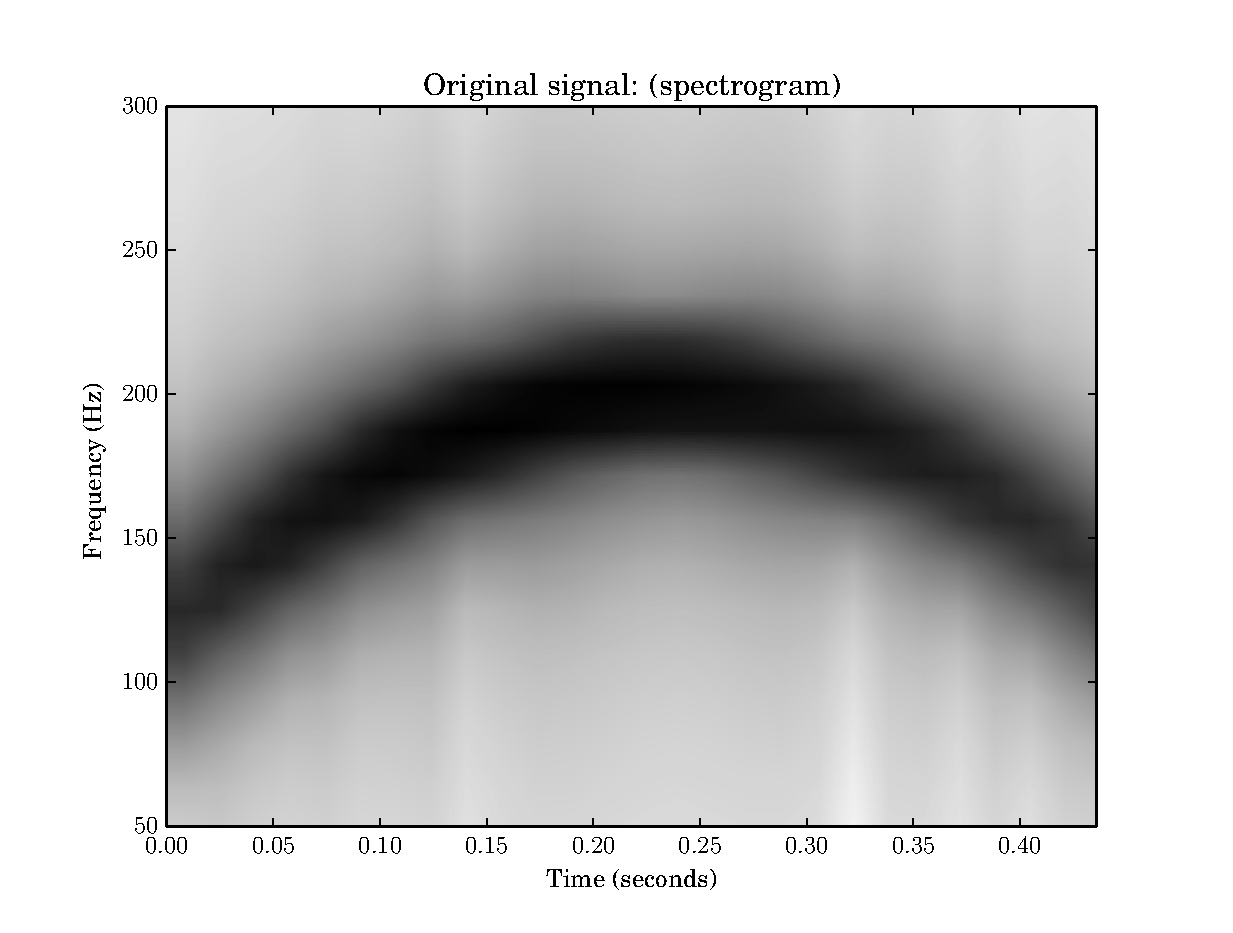
\includegraphics[width=\textwidth]{plots/mq_cubic_original_spec.eps}
    \caption{This depicts the log spectrum. Darker regions represent greater
        values whereas lighter are smaller values.
    \label{plot:mqcubicoriginalspec}}
\end{figure}

\begin{figure}
    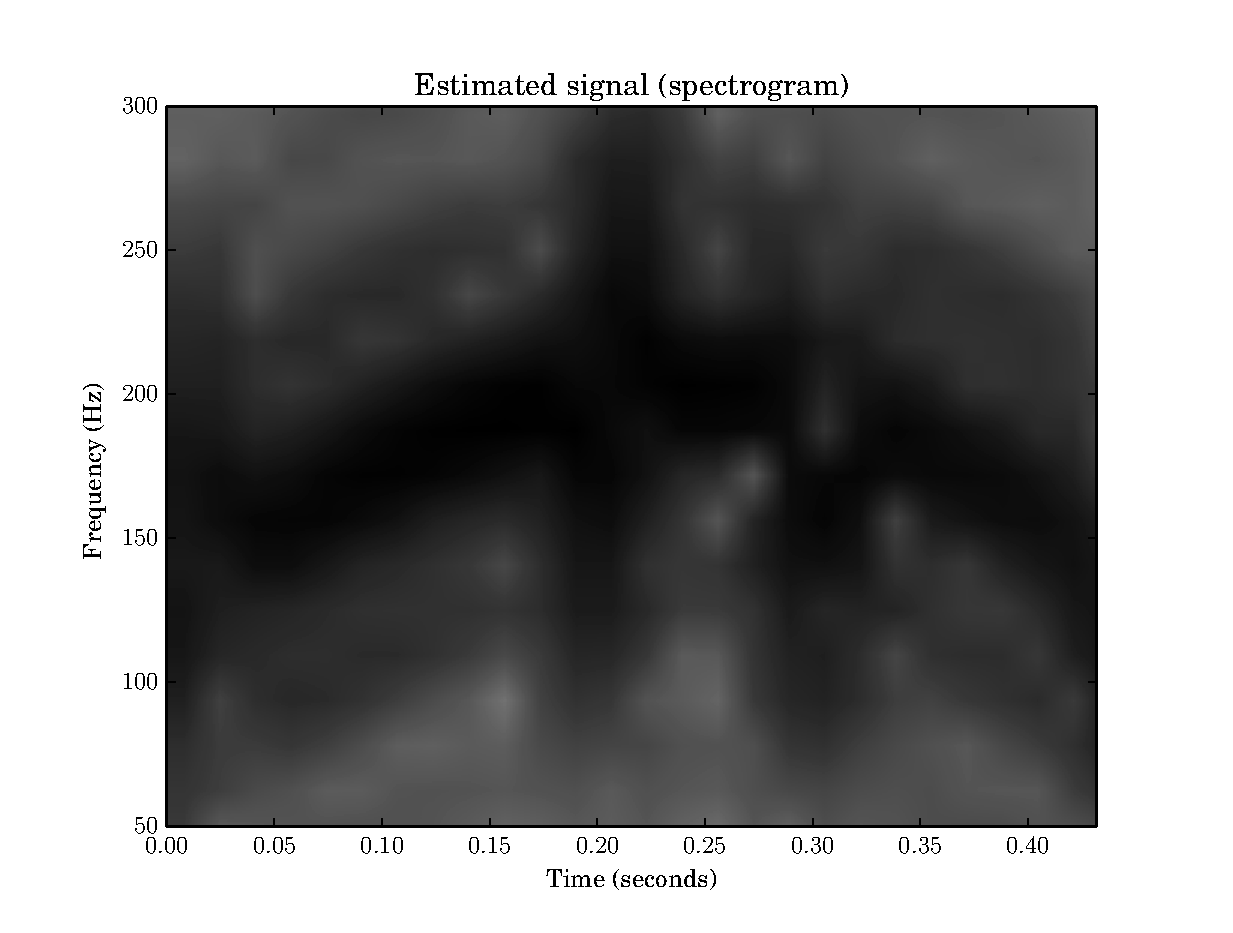
\includegraphics[width=\textwidth]{plots/mq_cubic_estimated_spec.eps}
    \caption{This depicts the log spectrum. Darker regions represent greater
        values whereas lighter are smaller values. The estimated signal is
        computed using the original method proposed by McAulay and Quatieri.
    \label{plot:mqcubicestimatedspec}}
\end{figure}

\begin{figure}
    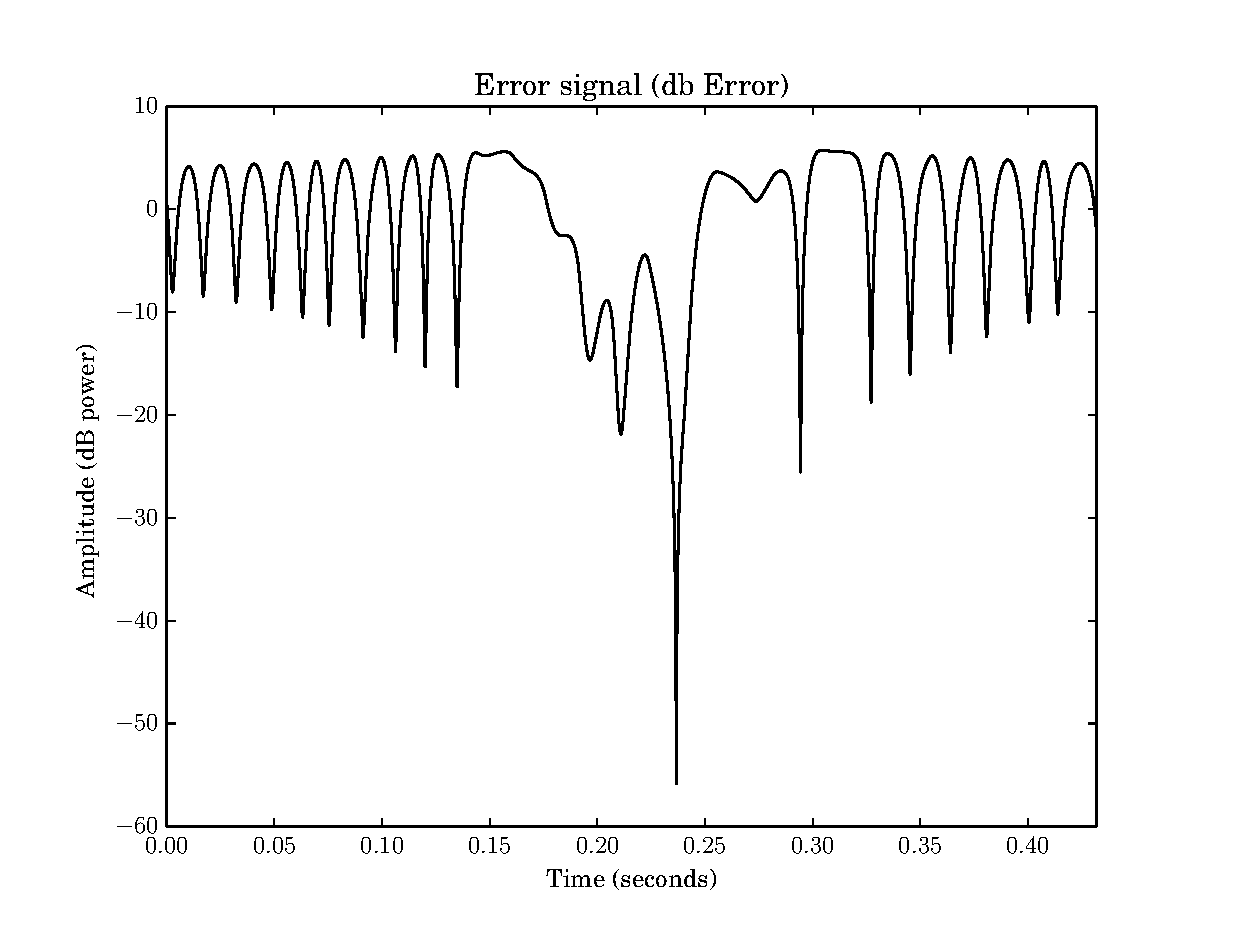
\includegraphics[width=\textwidth]{plots/mq_cubic_error.eps}
    \caption{
        The error when subtracting the original signal from the estimated
        signal. The estimated signal is computed using the original method
        proposed by McAulay and Quatieri.
    \label{plot:mqcubicerror}}
\end{figure}

%\begin{figure}
%    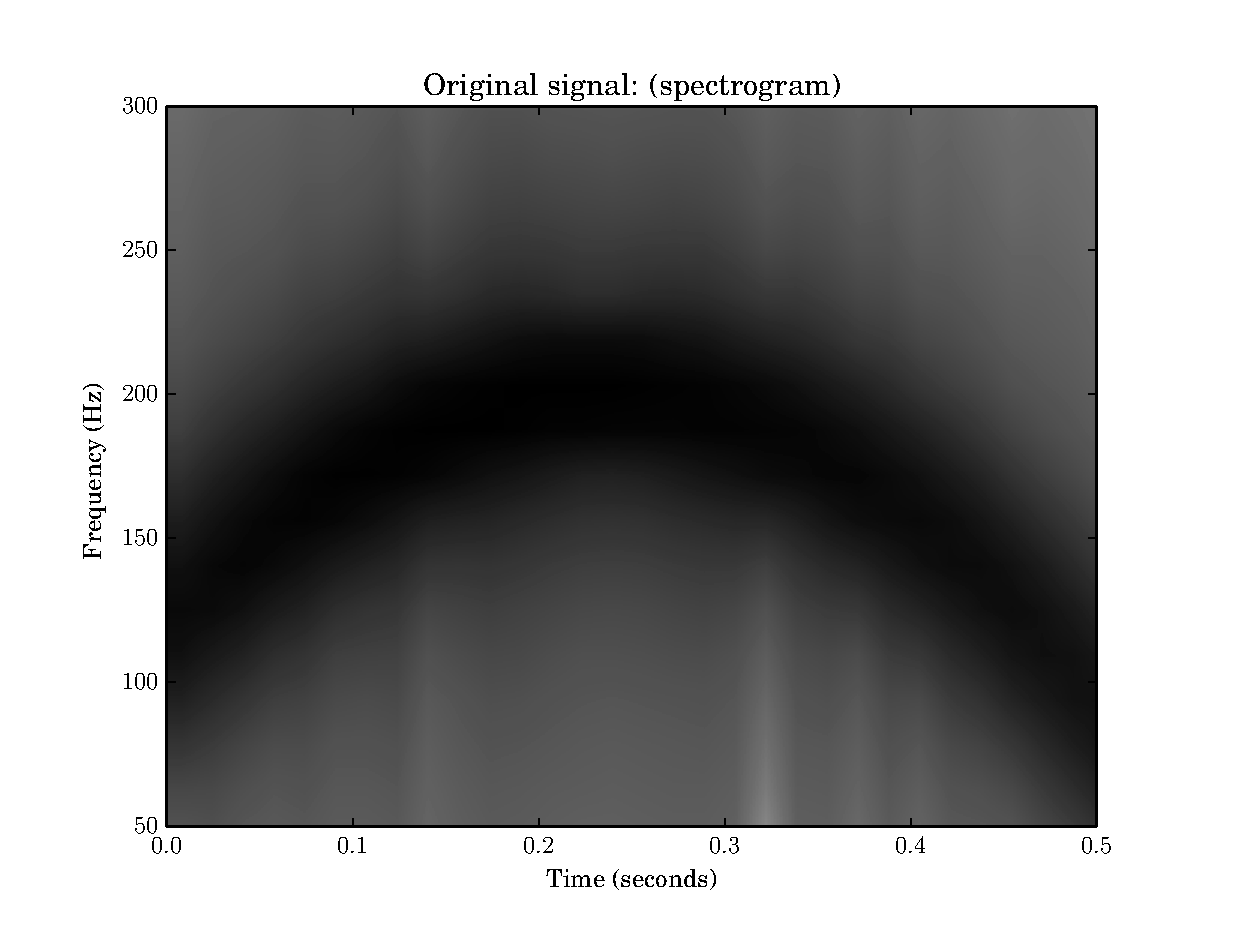
\includegraphics[width=\textwidth]{plots/mq_mod_cubic_original_spec.eps}
%    \caption{This depicts the dB spectrum. Darker regions represent greater
%        values whereas lighter are smaller values.
%    \label{plot:mqmodcubicoriginalspec}}
%\end{figure}

\begin{figure}
    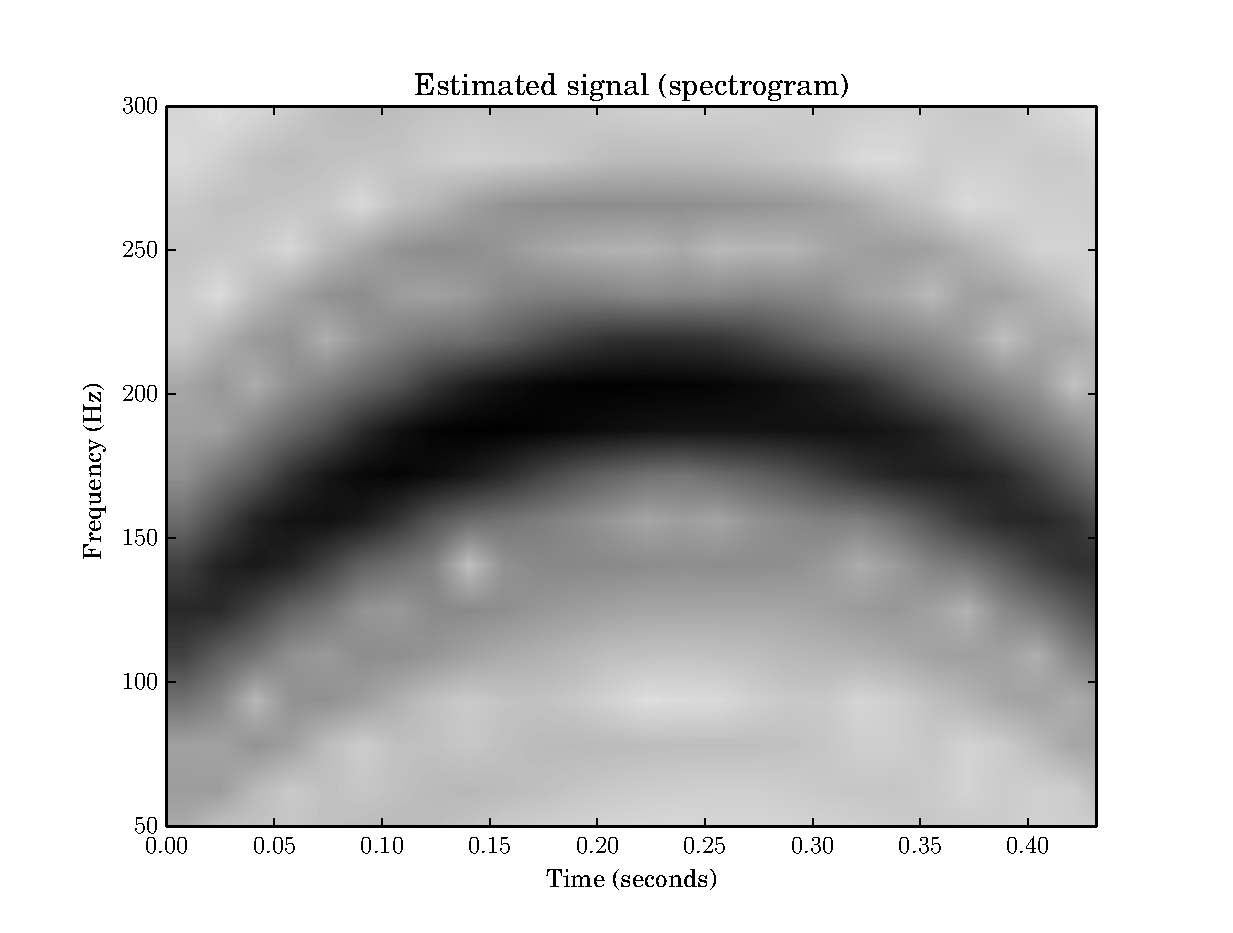
\includegraphics[width=\textwidth]{plots/mq_mod_cubic_estimated_spec.eps}
    \caption{This depicts the dB spectrum. Darker regions represent greater
        values whereas lighter are smaller values. The estimated signal is
        computed using the cubic interpolation method proposed here.
    \label{plot:mqmodcubicestimatedspec}}
\end{figure}

\begin{figure}
    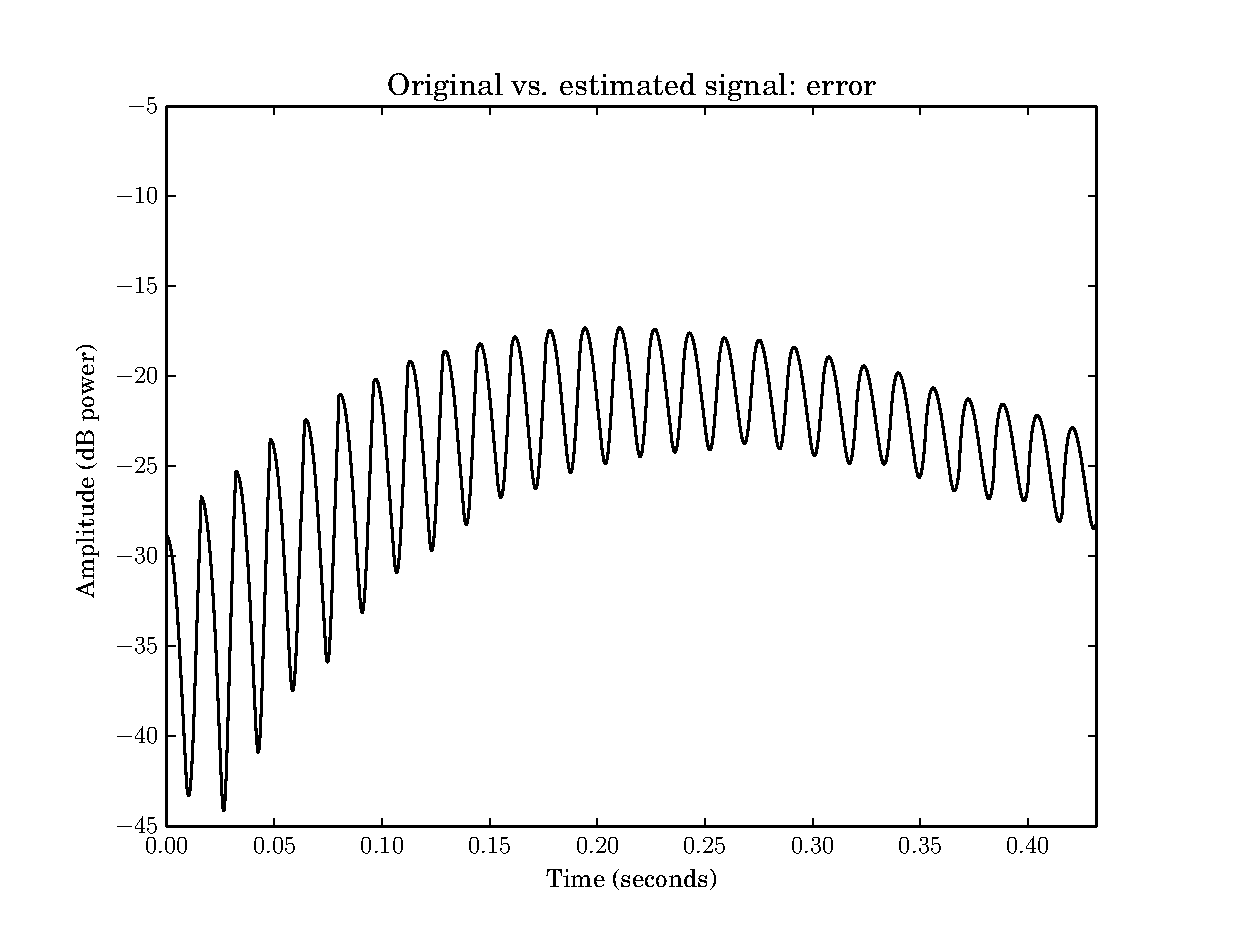
\includegraphics[width=\textwidth]{plots/mq_mod_cubic_error.eps}
    \caption{The error when subtracting the original signal from the estimated
        signal. The estimated signal is computed using the cubic interpolation
        method proposed here.
    \label{plot:mqmodcubicerror}}
\end{figure}

%\begin{figure}
%    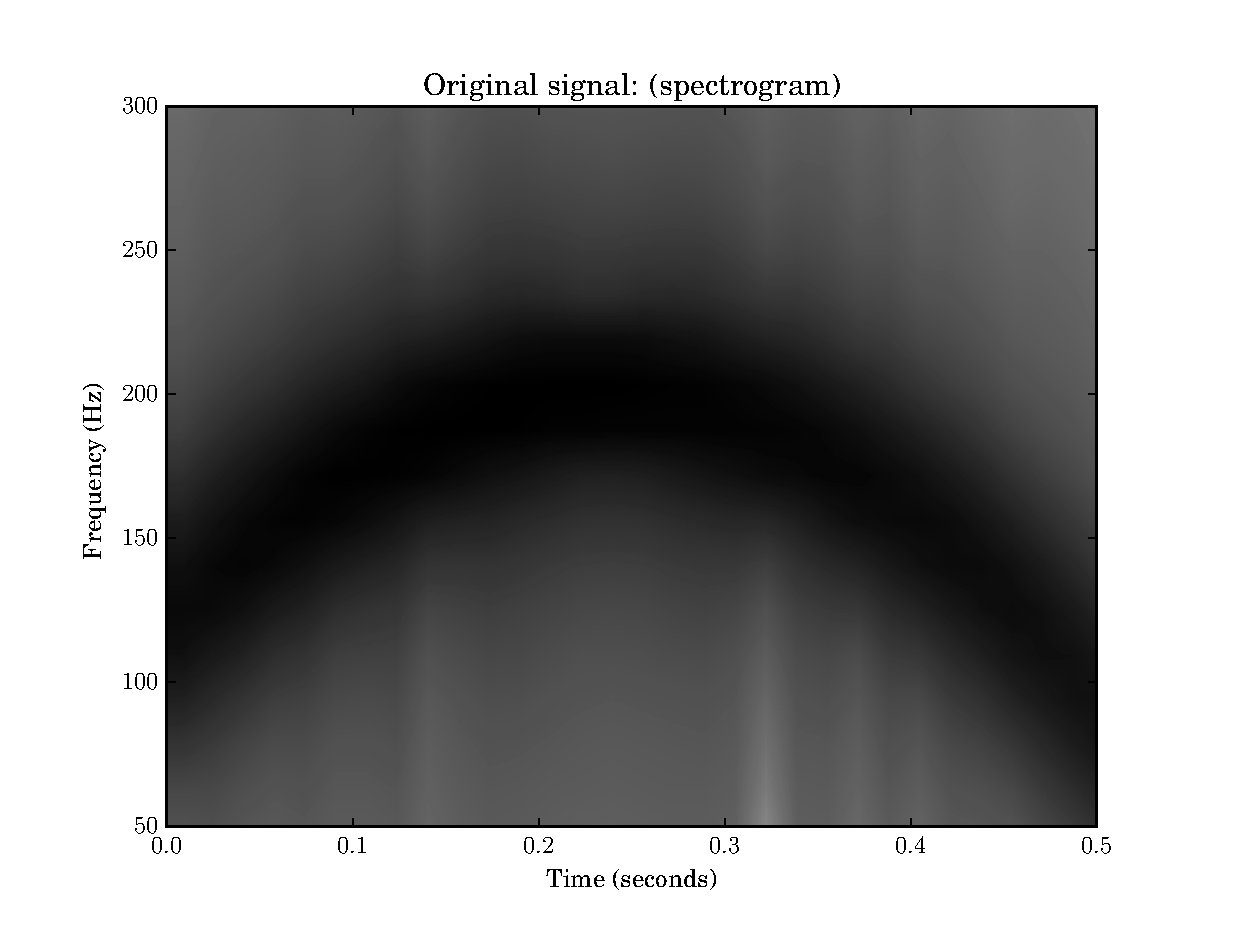
\includegraphics[width=\textwidth]{plots/mq_mod_quintic_original_spec.eps}
%    \caption{This depicts the dB spectrum. Darker regions represent greater
%        values whereas lighter are smaller values.
%    \label{plot:mqmodcubicoriginalspec}}
%\end{figure}

\begin{figure}
    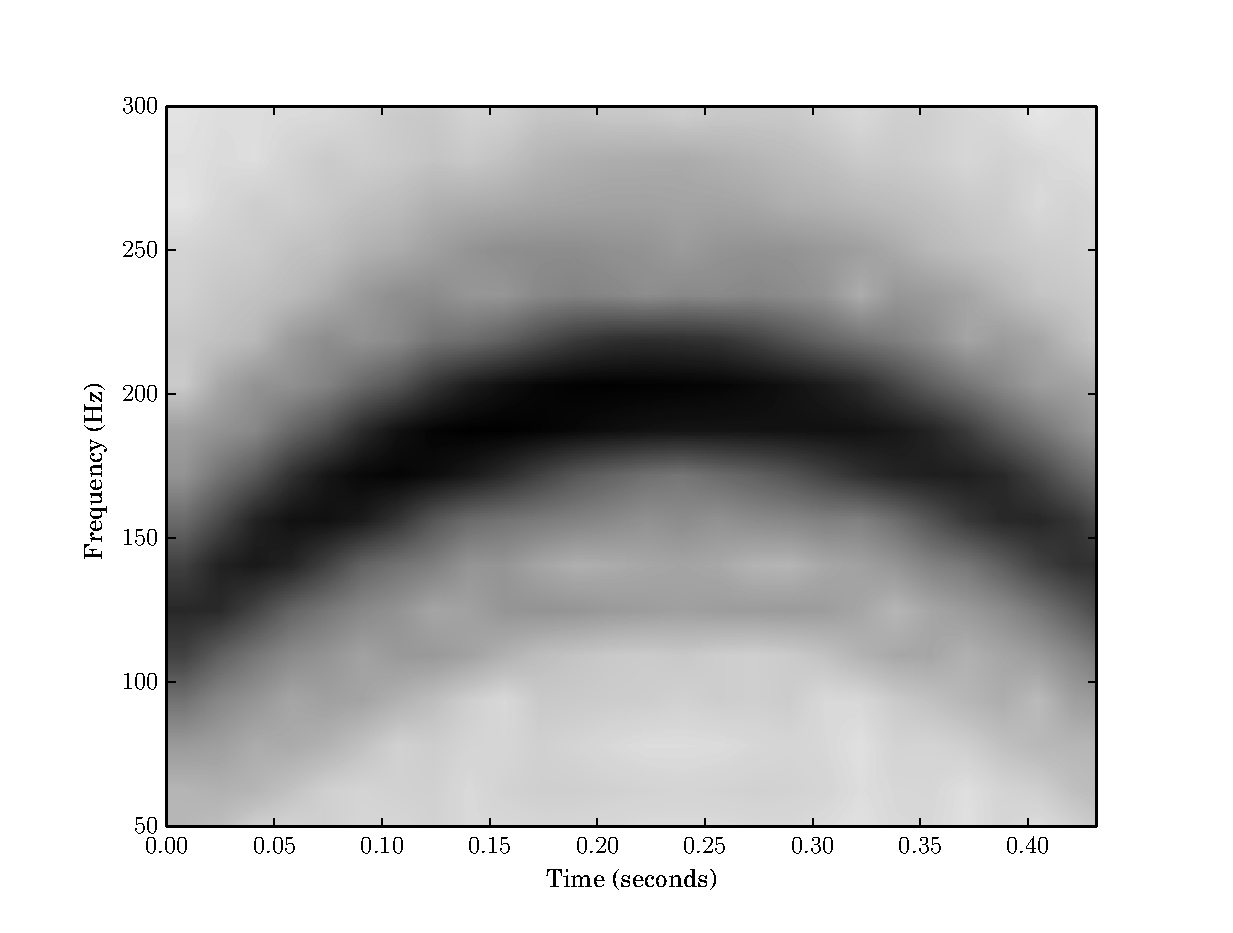
\includegraphics[width=\textwidth]{plots/mq_mod_quintic_estimated_spec.eps}
    \caption{This depicts the dB spectrum. Darker regions represent greater
        values whereas lighter are smaller values. The estimated signal is
        computed using the quintic interpolation method proposed here.
    \label{plot:mqmodcubicestimatedspec}}
\end{figure}

\begin{figure}
    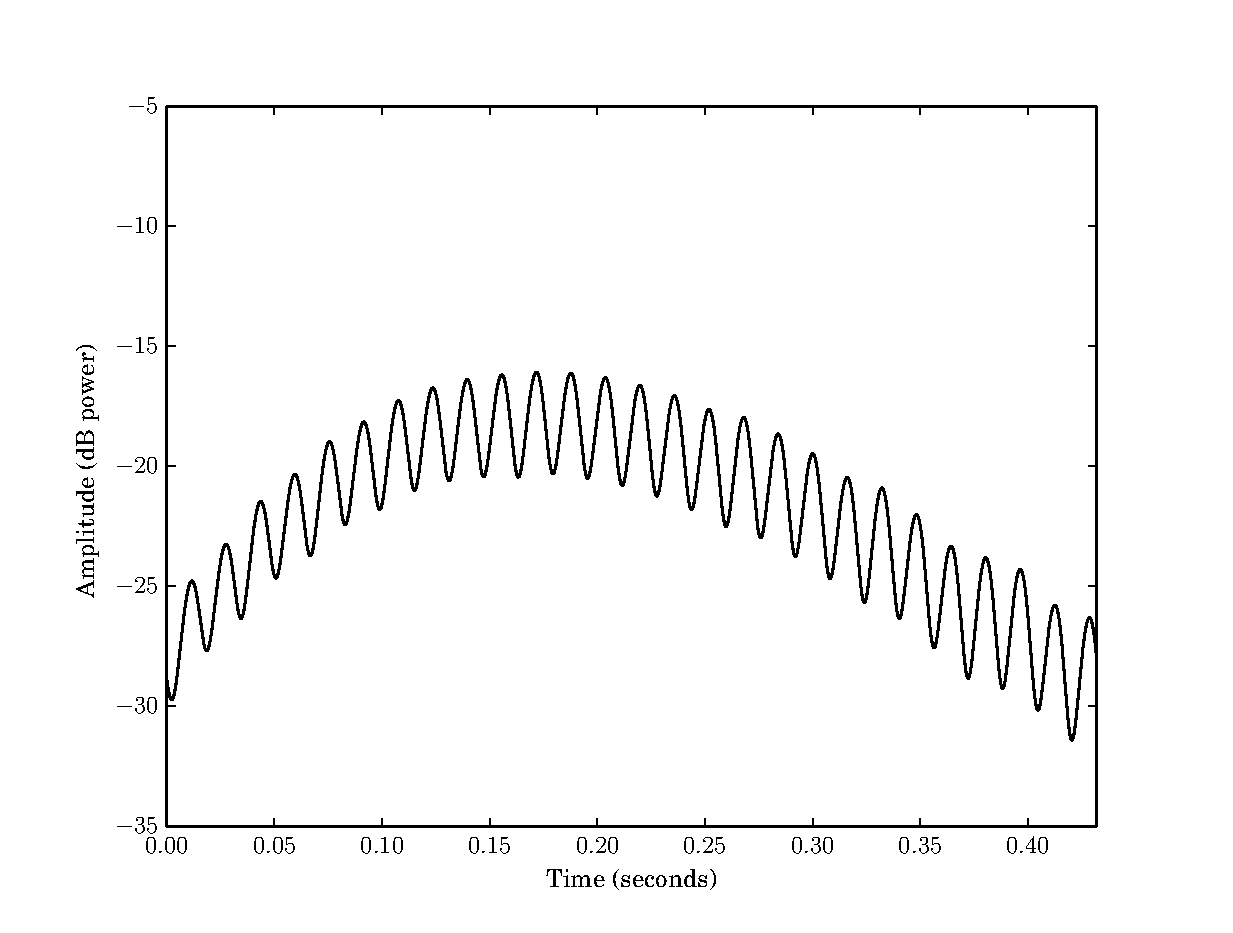
\includegraphics[width=\textwidth]{plots/mq_mod_quintic_error.eps}
    \caption{The error when subtracting the original signal from the estimated
        signal. The estimated signal is computed using the quintic interpolation
        method proposed here.
    \label{plot:mqmodcubicerror}}
\end{figure}

\begin{figure}
    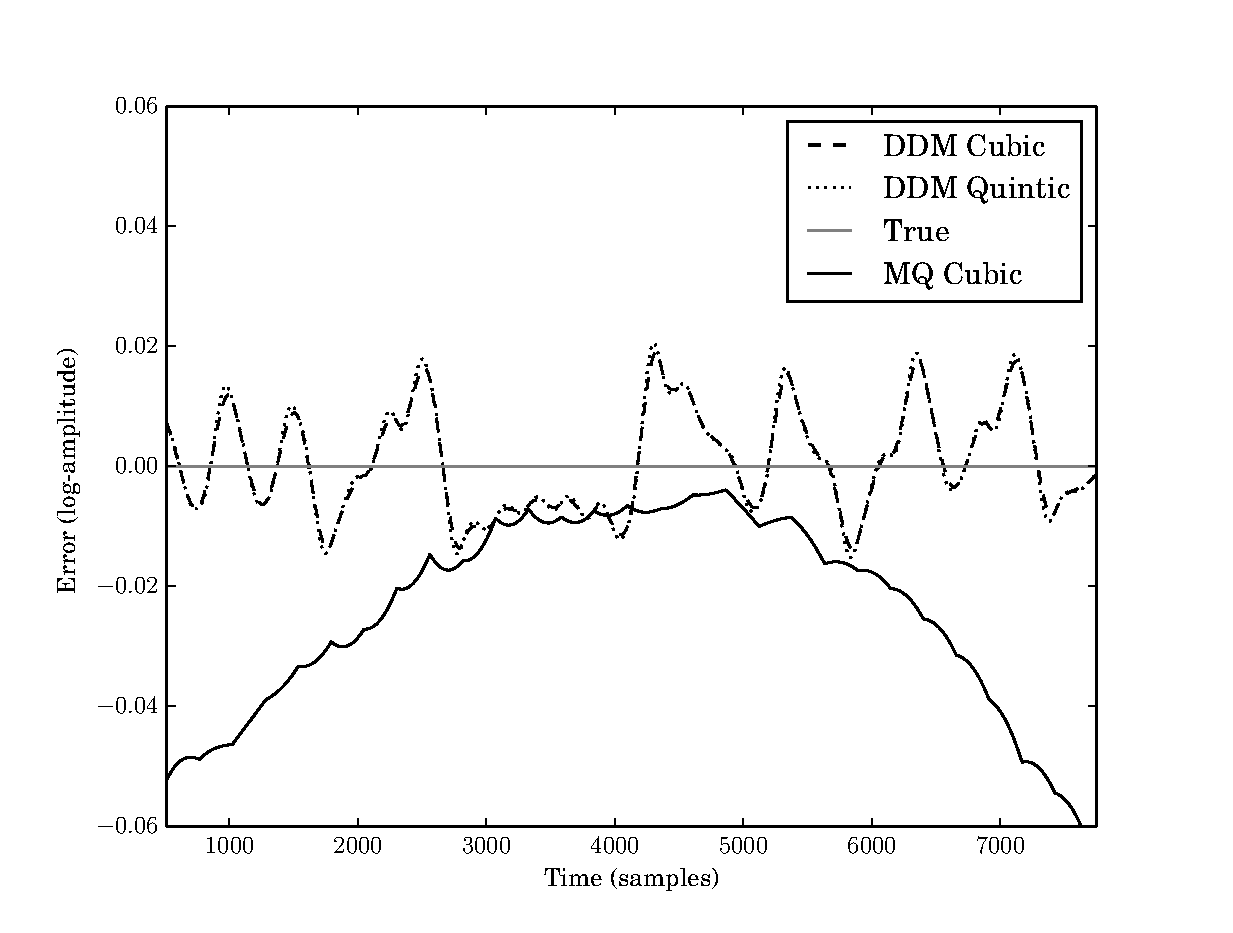
\includegraphics[width=\textwidth]{plots/mq_mod_err_comp_logamp_err.eps}
    \caption{This shows the error of the interpolated signals when compared
    with the original signal for the three proposed methods.
    \label{plot:mqmoderrcomplogamperr}}
\end{figure}

\begin{figure}
    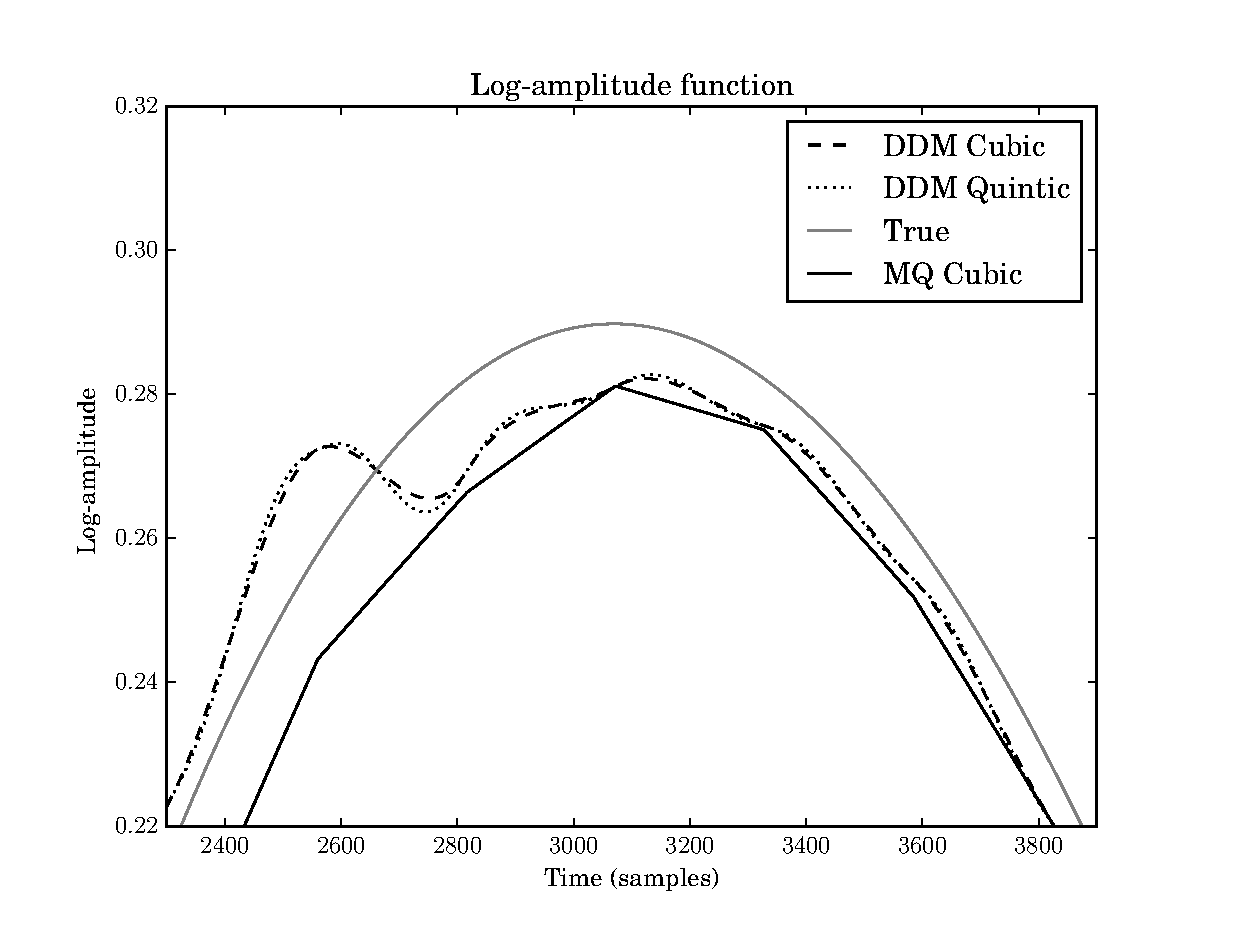
\includegraphics[width=\textwidth]{plots/mq_mod_err_comp_logamp_func.eps}
    \caption{This compares the original log-amplitude function with the
    interpolated log-amplitude functions. The log-amplitude functions are
    considered because these are the real part of the polynomial exponents in
    the complex sinusoid model.
    \label{plot:mqmoderrcomplogampfunc}}
\end{figure}

\begin{figure}
    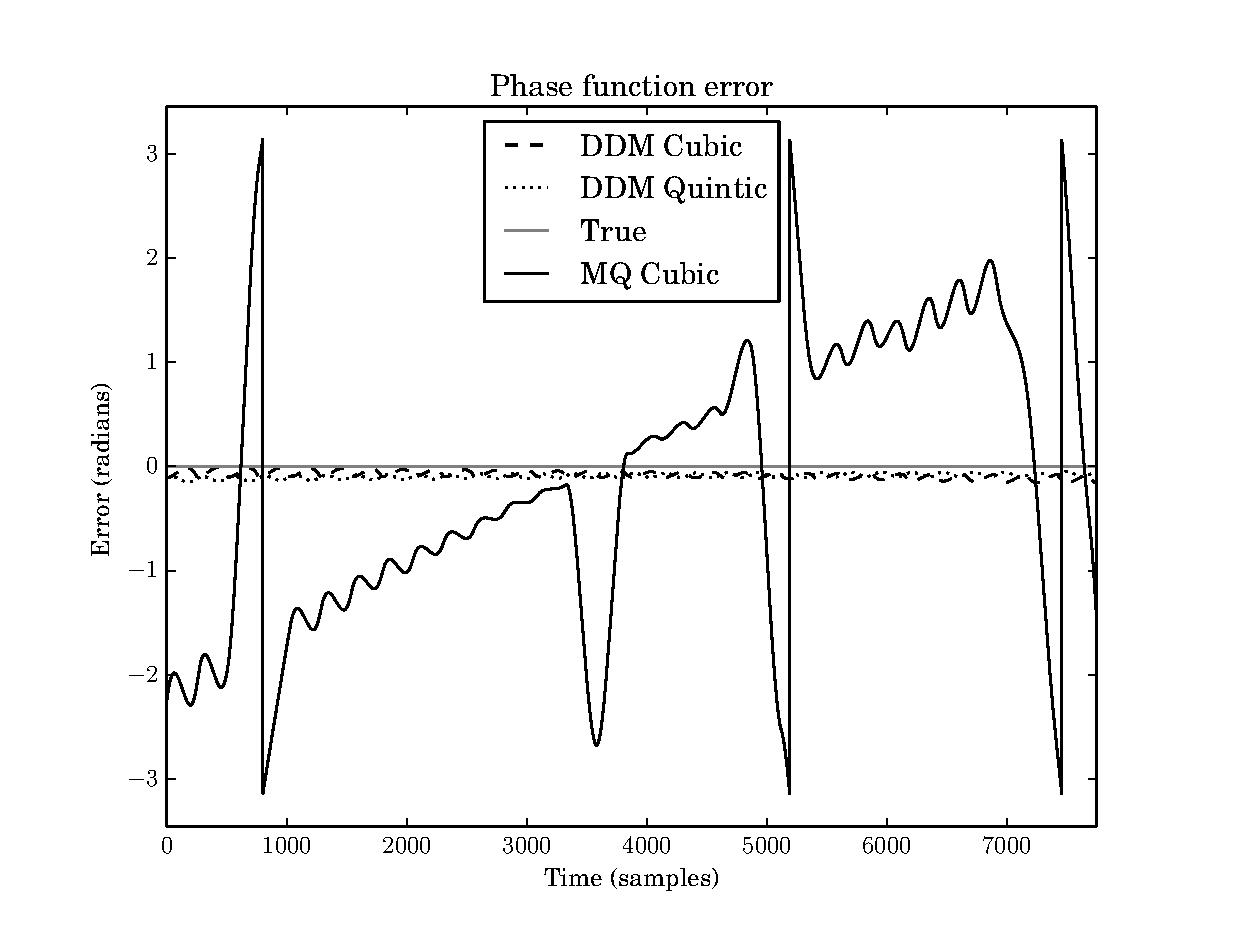
\includegraphics[width=\textwidth]{plots/mq_mod_err_comp_phase_err.eps}
    \caption{This compares the phase functions with the interpolated phase
    functions. The phase functions are considered because these are the
    imaginary part of the polynomial exponents in the complex sinusoidal model.
    The error exhibited by the McAulay \textendash Quatieri interpolation is
    misleading because phase values should be compared after computing the
    remaineder when dividing by $2\pi$. This means there are only brief segments
    where the phase error is significant (compare with
    Figure~\ref{plot:mqcubicerror}). The plot is shown without adjusting the
    values to show the accuracy of the proposed methods in the interpolated
    regions.
    \label{plot:mqmoderrcompphaseerr}}
\end{figure}

\begin{figure}
    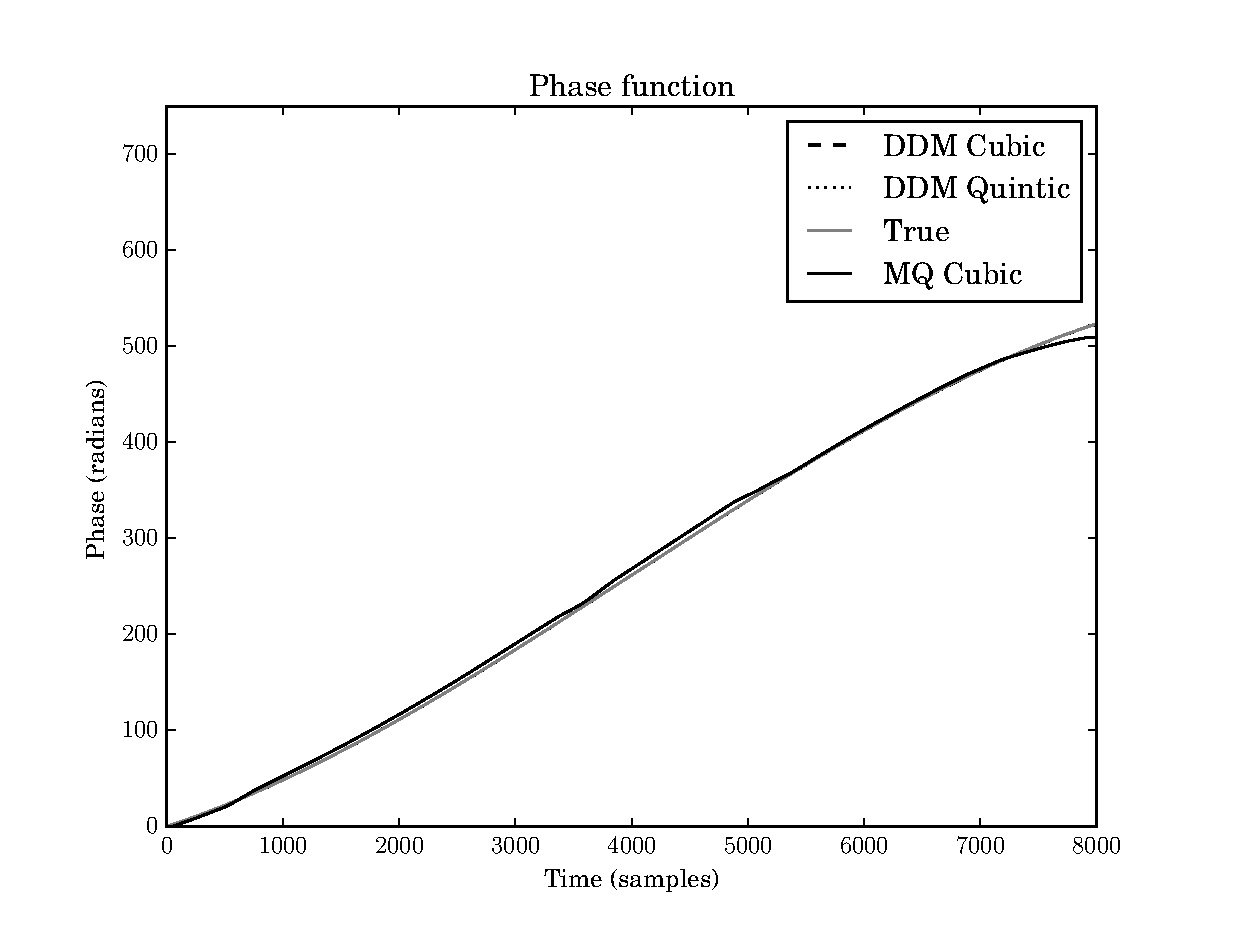
\includegraphics[width=\textwidth]{plots/mq_mod_err_comp_phase_func.eps}
    \caption{\label{plot:mqmoderrcompphasefunc}}
\end{figure}

\section{Conclusion}

Out of the three proposed methods it appears that the modified cubic
interpolation method works superiorily for the signal model considered. The
reduced accuracy of the higher-order quintic model can perhaps be explained by
the ``overfitting'' of the log-amplitude function (see
Figure~\ref{plot:mqmoderrcomplogampfunc}). Indeed, even the proposed cubic model
shows some overfitting in this case. From Figure~\ref{plot:mqmoderrcompphaseerr}
it is clear that the DDM based methods provide superior estimation of the phase
function---this is not the case for the log-amplitude function. Depending on
the underlying signal, perhaps better results can be obtained by postulating a
lower-order amplitude function and higher-order phase function. The possiblity
of errors arising from numerical accuracy when evaluating the quintic
polynomials has been ruled out. We evalutated these polynomials using an
implementation of Horner's method that keeps track of the error bound
\cite[p.~95]{higham2002accuracy}: the
errors are negligible, see Figure~\ref{plot:mqmodquinticpolyevalerr} for the
results.

\begin{figure}
    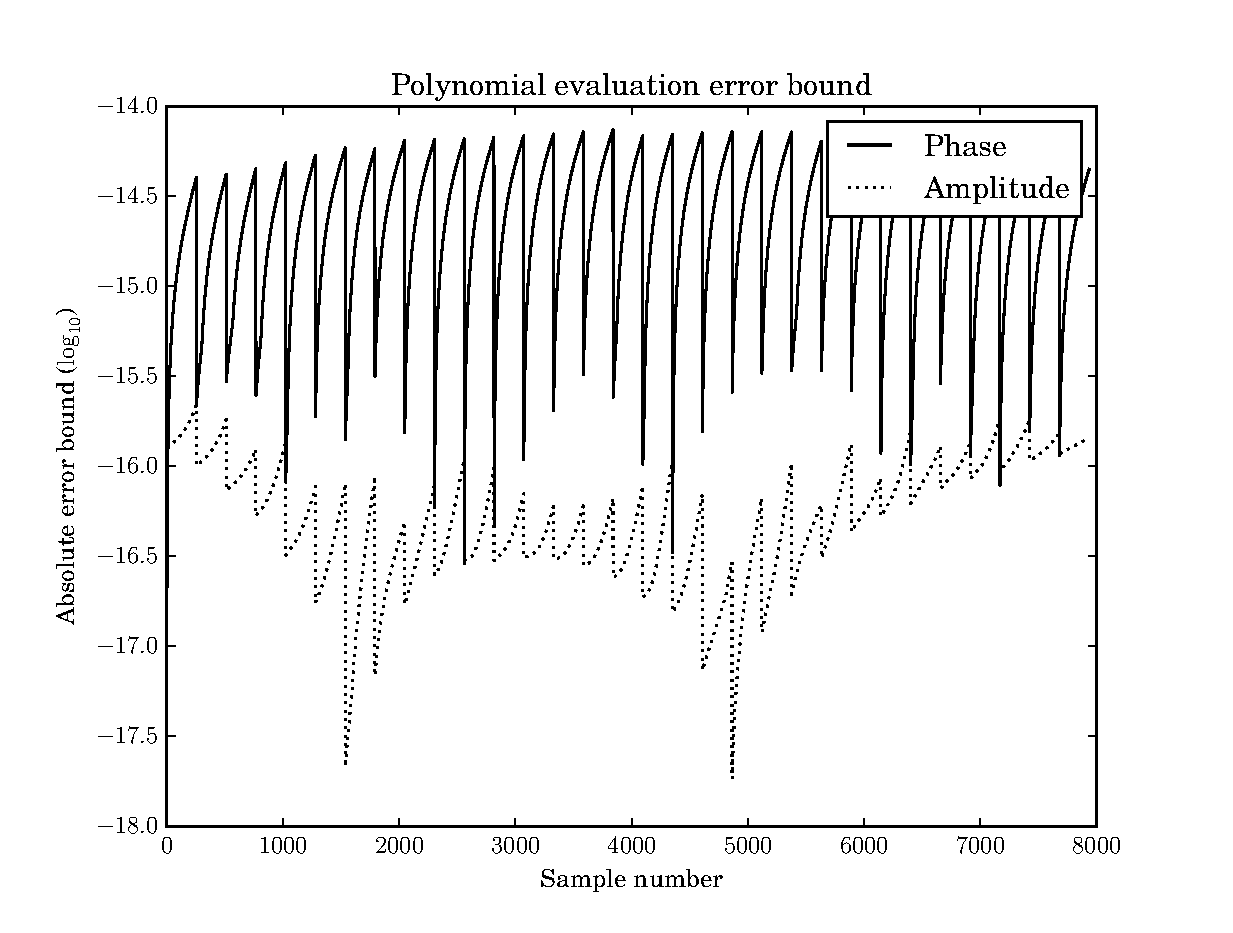
\includegraphics[width=\textwidth]{plots/mq_mod_quintic_poly_eval_err.eps}
    \caption{\label{plot:mqmodquinticpolyevalerr}}
\end{figure}
